% DRAFT: New Discussion subsection for Coherence Time paper
% To be added after "Biological examples of the speed-flexibility trade-off"
% Add when revisions requested
%
% Required packages (add to main document preamble if not present):
% \usepackage{float}    % For [H] figure placement
% \usepackage{graphicx} % For \includegraphics
%
% Figure files needed in figures/ directory:
% - cerebellar_takens_degradation.pdf (generated by simulations/cerebellar_takens_sim.py)

\subsection{How slow oscillations carry high-dimensional programs: delay embedding}

\begin{center}
\fbox{\parbox{0.95\textwidth}{
\textbf{Takens Mapping (Formal Statement)}\\[0.5em]
\textbf{State:} $\mathbf{s}(t) \in \mathbb{R}^d$ --- high-dimensional motor/coordination dynamics\\
\textbf{Observable:} $y(t) = h(\mathbf{s}(t))$ --- scalar projection (e.g., cortical efference copy, error signal)\\
\textbf{Delay embedding:} $\mathbf{Y}(t) = [y(t), y(t-\tau), y(t-2\tau), \ldots, y(t-(m-1)\tau)]$\\
\textbf{Theorem (Takens, 1981):} For generic $h$ and $\tau$, if $m \geq 2d+1$, then $\mathbf{Y}(t)$ is diffeomorphic to $\mathbf{s}(t)$.\\[0.5em]
\textbf{Biological hypothesis:} The observable $y(t)$ is the descending cortical command/error signal distributed via mossy fibers; parallel fiber delays provide the $\tau_1, \tau_2, \ldots$ taps; Purkinje dendritic integration forms $\mathbf{Y}(t)$.
}}
\end{center}

The speed-flexibility trade-off explains \emph{when} oscillatory assemblies can commit, but not \emph{how} slow oscillations encode the high-dimensional programs they coordinate. We propose that biological systems implement \textbf{Takens delay embedding}---a mathematical technique for reconstructing high-dimensional dynamics from scalar time series~\cite{takens1981}.

\paragraph{Takens' theorem.}
For a deterministic system with state dimension $d$, Takens proved that time-delayed copies of a scalar observable---$x(t), x(t-\tau), x(t-2\tau), \ldots$---can reconstruct the complete state-space topology. Crucially, $2d+1$ delay coordinates generically suffice. This means a low-frequency ``carrier'' signal, properly sampled across delays, contains complete information about arbitrarily complex dynamics.

\paragraph{Robustness to noise and nonstationarity.}
Takens' theorem is asymptotic and assumes deterministic dynamics. Biological systems are noisy, adaptive, and nonstationary. We therefore use Takens embedding as a \emph{design principle} rather than a literal guarantee: delay-line architectures improve state inference under partial observability, even when exact reconstruction is impossible. In noisy regimes, the claim becomes: systems with delay-diverse sampling achieve higher mutual information between observations and underlying state than systems with instantaneous-only sampling. This weaker claim is empirically testable and does not require deterministic dynamics.

\paragraph{Biological implementation: cerebellar parallel fibers.}
The cerebellum provides a striking biological realization. Parallel fibers---unmyelinated granule cell axons---conduct at 0.2--0.5 m/s with systematically varying path lengths, creating conduction delays of 10--23 ms~\cite{braitenberg1958,llinas1982}. These delays match the optimal embedding parameter $\tau^* \approx 1/(4f)$ for motor error signals at 10--25 Hz.

We hypothesize that the relevant observable $y(t)$ is the descending cortical efference copy or sensorimotor prediction error, broadcast broadly via mossy fiber inputs. Parallel fiber delays then provide the temporal basis $\{y(t-\tau_i)\}$, and Purkinje cell dendritic integration computes a readout over this delay-expanded representation. The cerebellum is not merely timing movements---it is reconstructing state from delay-embedded observations.

\paragraph{Why ferns and Purkinje cells look the same.}
Purkinje cell dendritic arbors exhibit ``fern-leaf'' fractal geometry remarkably similar to botanical ferns. Both structures involve low-dimensional channels operating on high-dimensional spaces: ferns are fractal as a byproduct of low-D GRN construction; Purkinje arbors are fractal-like because they must sample parallel fiber inputs across the full delay range for embedding. Different mechanisms, same geometric pattern---both show what low-D structures look like when embedded in high-D flows. (The testable claim concerns delays, not morphology.)

\paragraph{Simulation: degraded temporal structure destroys reconstruction.}
To test whether phase coherence (rather than amplitude) is the critical variable, we simulated Takens reconstruction under two forms of signal degradation: (1) phase jitter (timing noise without amplitude change) and (2) amplitude noise (conventional SNR degradation). Using a Lorenz attractor as ground-truth dynamics and measuring neighborhood preservation in the reconstructed manifold, we find:

\begin{itemize}
\item Phase jitter of 0.5 (normalized units) reduces reconstruction quality from 75\% to 37\%
\item The degradation is smooth and monotonic---no sharp threshold
\item Even moderate timing dysfunction impairs coordination before amplitude loss becomes obvious
\end{itemize}

Figure~\ref{fig:takens_degradation} shows the key result: reconstruction quality degrades smoothly with phase jitter. The attractor structure progressively dissolves (panels d--f), becoming unrecognizable at high jitter despite unchanged signal amplitude. This directly supports the clinical prediction: coordination fails when temporal structure degrades, not when cells die.

\begin{figure}[H]
\centering
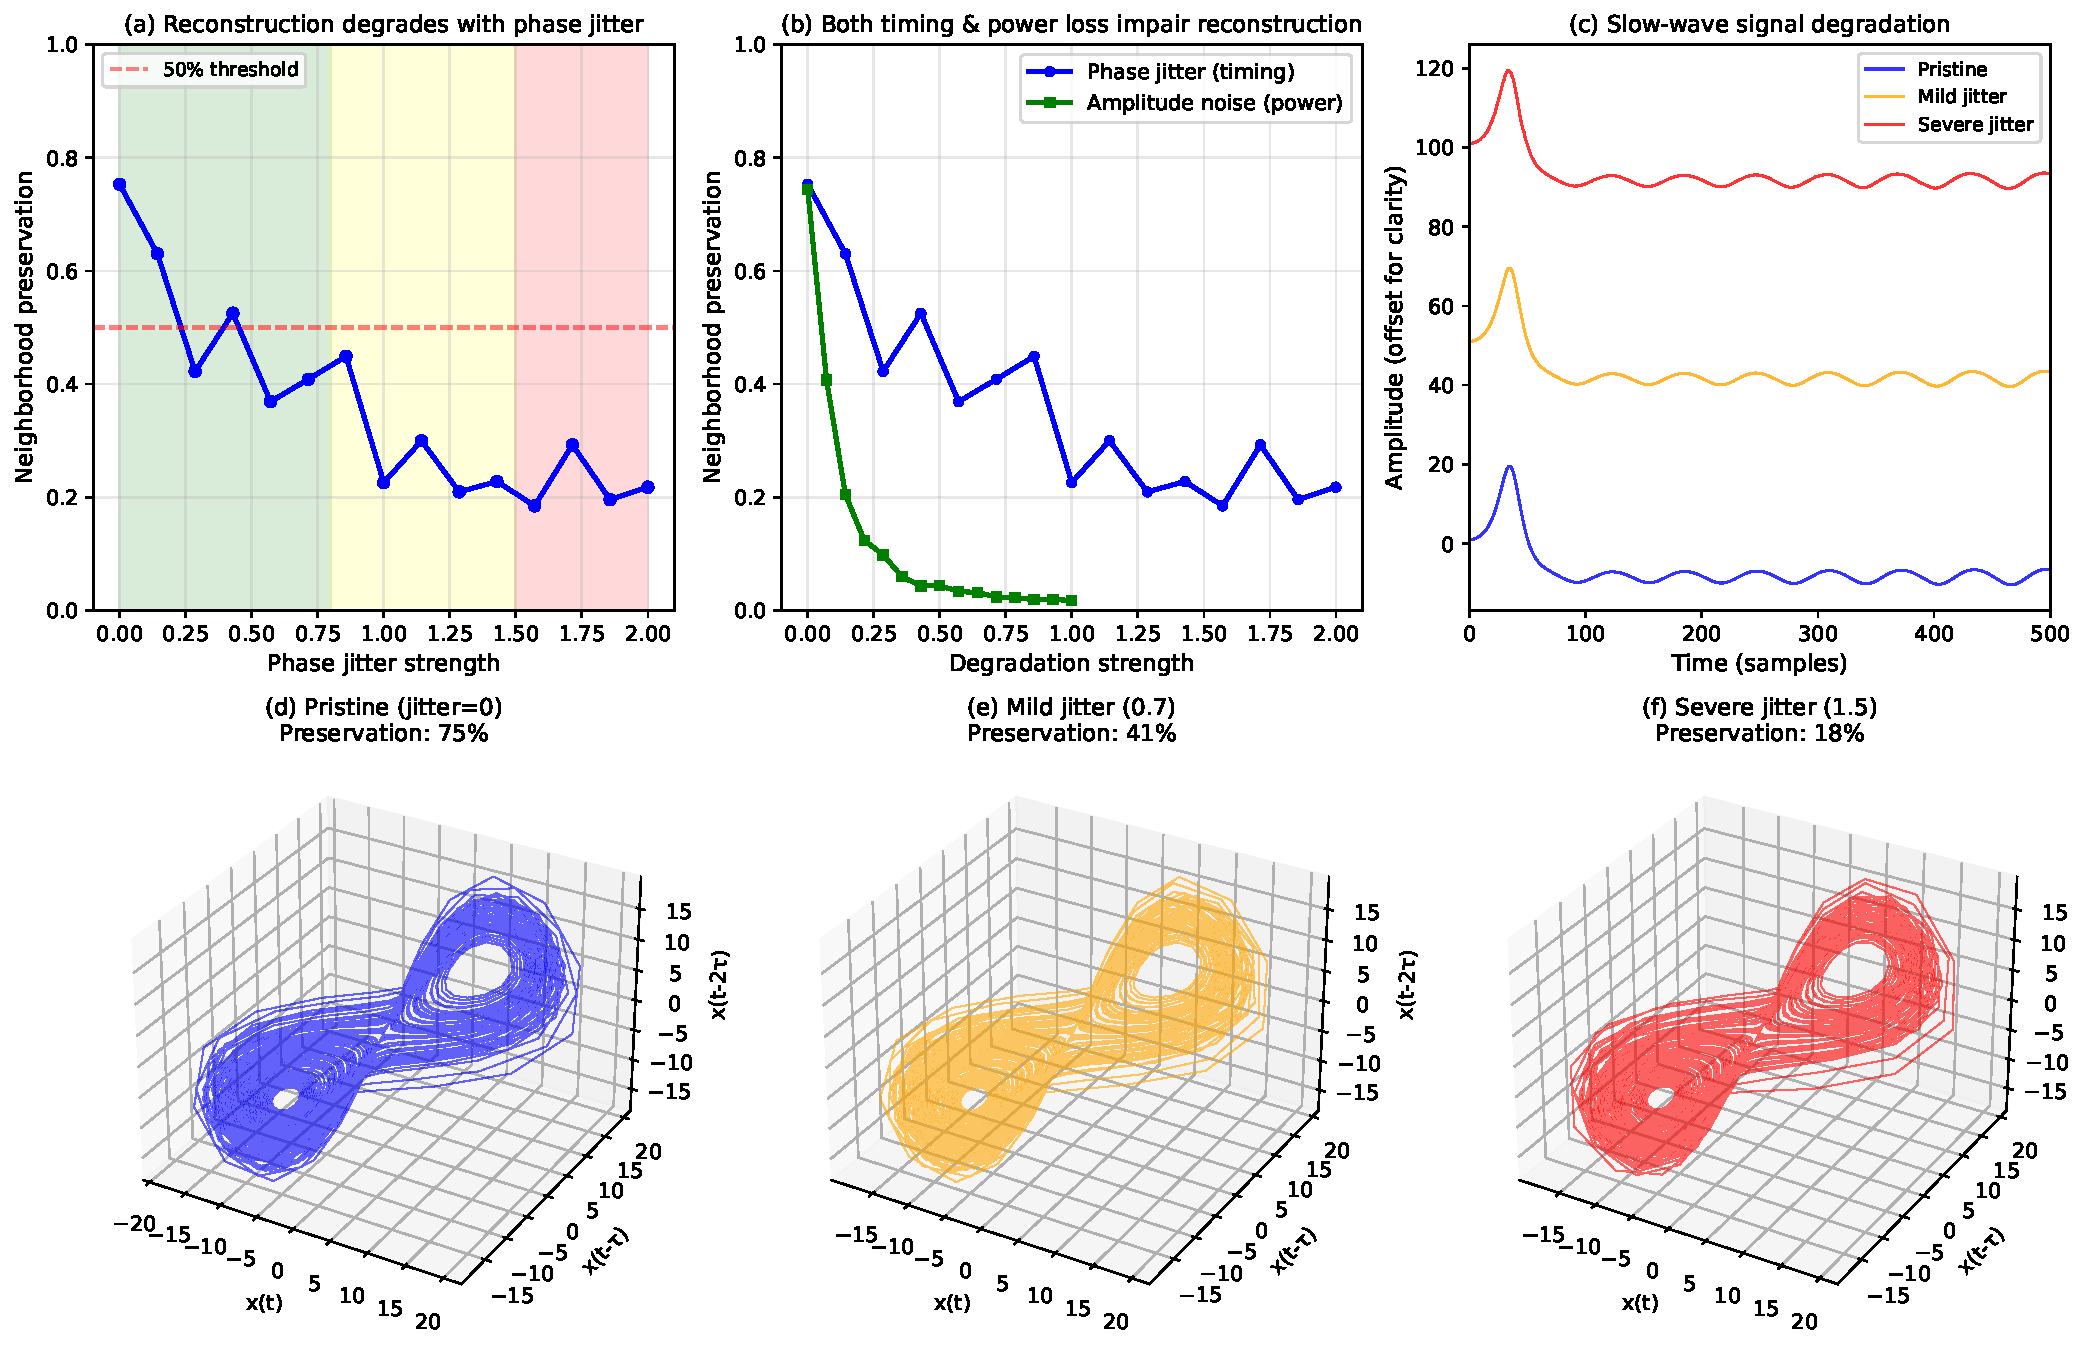
\includegraphics[width=\textwidth]{figures/cerebellar_takens_degradation.pdf}
\caption{\textbf{Degraded slow-wave structure destroys Takens reconstruction.} (a) Neighborhood preservation declines smoothly with phase jitter. (b) Both timing and amplitude degradation impair reconstruction. (c) Example signals at different jitter levels. (d--f) Reconstructed attractors: pristine (d), mild jitter (e), and severe jitter (f). The attractor structure dissolves progressively---coordination fails before amplitude loss.}
\label{fig:takens_degradation}
\end{figure}

\paragraph{Connection to coherence time.}
Takens embedding explains \emph{what} slow oscillations carry; coherence time explains \emph{when} that information can be read out. The two frameworks are complementary:

\begin{itemize}
\item Slow oscillations encode high-dimensional programs via delay embedding
\item Fast oscillations (gamma) provide the readout/execution layer
\item Phase-amplitude coupling links the two: slow phases gate when fast activity can commit
\item Coherence time determines the minimum interval between commits
\end{itemize}

When slow-wave temporal structure degrades---through pathology, fatigue, or pharmacological disruption---the delay-embedded program becomes unreadable even if signal amplitude is preserved. This predicts that \emph{phase coherence}, not just oscillation power, should correlate with coordination capacity.

\paragraph{Clinical implication.}
Conditions disrupting slow-wave coordination (motor neuron disease, cerebellar ataxia, sleep deprivation) may impair function not through cell loss but through loss of reconstructible temporal structure. Therapeutic interventions preserving phase relationships may be as important as those preserving amplitude.

% References to add:
% \bibitem[Takens, 1981]{takens1981}
% Takens, F. (1981). Detecting strange attractors in turbulence.
% In: Rand, D., Young, L.S. (eds) Dynamical Systems and Turbulence.
% Lecture Notes in Mathematics, vol 898. Springer.
%
% \bibitem[Braitenberg, 1958]{braitenberg1958}
% Braitenberg, V. (1958). Morphology of nerve net in cerebellar cortex.
% Journal of Comparative Neurology, 109, 1--33.
%
% \bibitem[Llinás, 1982]{llinas1982}
% Llinás, R. (1982). General discussion: Radial connectivity in the cerebellar cortex.
% In: The Cerebellum---New Vistas (pp. 189--194). Springer.
